\documentclass{beamer}

\usepackage{amsmath}
\usepackage{cancel}
\usepackage{mathtools}
\usepackage{multirow}
\usepackage{tikz, pgfplots}
\pgfplotsset{compat=1.18}

\title{Applying the Klein-Gordon Theory to Gravitation}

\subtitle{Modelling Newtonian gravitation as a classical scalar field theory obeying Klein-Gordon structure}

\author{Siddhartha Bhattacharjee}

\institute
{
1B Mathematical Physics \\
University of Waterloo
}

\date{SASMS, Feb 10, 2023}

\begin{document}

\frame{\titlepage}

\begin{frame}
\begin{center}
\huge \textcolor{blue!50!gray}{Towards Classical Field Theory}
\end{center}
\end{frame}

\begin{frame}
\frametitle{The Inverse Square Law}

\begin{itemize}
\item Gravitational force:
\end{itemize}

$$F_m = - G \frac{M m}{r^2}$$

\begin{itemize}
\item Electrostatic force:
\end{itemize}

$$F_e = \frac{1}{4 \pi \epsilon_0} \frac{Q_e q_e}{r^2}$$

\begin{itemize}
\item Magnetic force:
\end{itemize}

$$F_b = \frac{\mu_0}{4 \pi} \frac{Q_b q_b}{r^2}$$
\end{frame}

\begin{frame}
\frametitle{Formal Analogies Between the Gravitational and Electrostatic Forces}

\begin{center}
\begin{tabular}{ |c|c|c|c| } 
\hline
& Gravitation & Static electricity \\
\hline
Newton's second law & $a^i = \underset{- \vec{\nabla} V}{\underbrace{- \partial^i V}}$ & $E^i = \underset{- \vec{\nabla} \phi}{\underbrace{- \partial^i \phi}}$ \\
\hline
Gauss' law & $\underset{\vec{\nabla} \cdot \vec{a}}{\underbrace{\sum \limits_{i=1}^3 \nabla_i a^i}} = - 4 \pi G \rho_m$ & $\underset{\vec{\nabla} \cdot \vec{a}}{\underbrace{\sum \limits_{i=1}^3 \nabla_i E^i}} = \frac{1}{\epsilon_0} \rho_e$ \\
\hline
Poisson's equation & $\underset{\nabla^2 V}{\underbrace{\sum \limits_{i=1}^3 \nabla_i \partial^i V}} = 4 \pi G \rho_m$ & $\underset{\nabla^2 \phi}{\underbrace{\sum \limits_{i=1}^3 \nabla_i \partial^i \phi}} = - \frac{1}{\epsilon_0} \rho_e$ \\  
\hline
\end{tabular}
\end{center}
\end{frame}

\begin{frame}
\frametitle{Lagrangian Mechanics}

\begin{center}
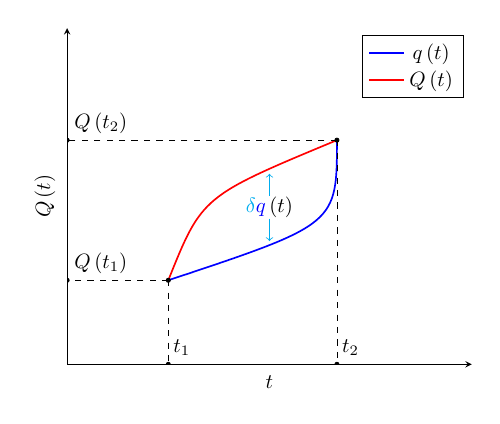
\begin{tikzpicture}[scale=0.75]
\begin{axis}[
    axis lines = left,
    xlabel = $t$,
    ylabel = $Q \left( t \right)$,
    xtick = \empty,
    ytick = \empty,
    xmin=0, xmax=3,
    ymin=0, ymax=3,
]

\draw[thick, blue] (0.75, 0.75) .. controls (2, 1.25) .. (2, 2);
\addlegendimage{thick, color=blue};
\addlegendentry{$q \left( t \right)$};

\draw[thick, red] (0.75, 0.75) .. controls (1, 1.5) .. (2, 2);
\addlegendimage{thick, color=red};
\addlegendentry{$Q \left( t \right)$};

\draw[->, color=cyan] (1.5, 1.5) to (1.5, 1.7);
\draw[->, color=cyan] (1.5, 1.3) to (1.5, 1.1);
\node[] at (1.5, 1.4) {$\textcolor{cyan}{\delta} \textcolor{blue}{q} \left( t \right)$};

\draw[dashed] (0.75, 0.75) -- (0.75, 0);
\draw[dashed] (0.75, 0.75) -- (0, 0.75);
\draw[dashed] (2, 2) -- (2, 0);
\draw[dashed] (2, 2) -- (0, 2);
\node[] at (0.85, 0.15) {$t_1$};
\node[] at (2.1, 0.15) {$t_2$};
\node[] at (0.25, 0.9) {$Q \left( t_1 \right)$};
\node[] at (0.25, 2.15) {$Q \left( t_2 \right)$};

\filldraw[] (0.75, 0.75) circle (1 pt);
\filldraw (2, 2) circle (1 pt);
\filldraw (0.75, 0) circle (1 pt);
\filldraw (0, 0.75) circle (1 pt);
\filldraw (2, 0) circle (1 pt);
\filldraw (0, 2) circle (1 pt);

\end{axis}
\end{tikzpicture}
\end{center}

\begin{itemize}
\item Nature 'selects' the unique on-shell trajectory $\textcolor{blue}{q \left( t \right)}$ given the boundary conditions $\left( t_1, \textcolor{red}{Q \left( t_1 \right)} \right)$ and $\left( t_2, \textcolor{red}{Q \left( t_2 \right)} \right)$ for a system.
\end{itemize}

\begin{align*}
\underset{\text{Off-shell}}{\underbrace{\textcolor{red}{Q \left( t \right)}}} & = \underset{\text{On-shell}}{\underbrace{\textcolor{blue}{q \left( t \right)}}} + \underset{\text{Variation}}{\underbrace{\textcolor{cyan}{\delta} \textcolor{blue}{q} \left( t \right)}} \\
\textcolor{cyan}{\delta} \textcolor{blue}{q \left( t_1 \right)} & = \textcolor{cyan}{\delta} \textcolor{blue}{q \left( t_2 \right)} = 0
\end{align*}
\end{frame}

\begin{frame}
\begin{itemize}
\item Each trajectory $\textcolor{red}{Q \left( t \right)}$ between the endpoints is associated with a corresponding number called the action.
\end{itemize}

$$\boxed{S \left[ \textcolor{red}{Q \left( t \right)} \right] \left( t_1, t_2 \right) = \int_{t_1}^{t_2} dt \: L \left( \textcolor{red}{Q \left( t \right)}, \textcolor{red}{\dot{Q} \left( t \right)}, t \right)}$$

\begin{flushright}
The integrand $L \left( \textcolor{red}{Q \left( t \right)}, \textcolor{red}{\dot{Q} \left( t \right)}, t \right)$ is known as the Lagrangian of the system being modelled and encodes the dynamics of the system.
\end{flushright}

\begin{itemize}
\item In general, the action $S$ maps $\textcolor{red}{Q \left( t \right)}$ to a real number determined by the above integral. Therefore, it is a functional, i.e. a higher-order function which takes in infinite values of the form $\left\{ \left( t, \textcolor{red}{Q \left( t \right)} \right) : t \in \mathbb{R} \right\}$ and spits out a real.
\end{itemize}

$$
S : \begin{cases} \mathbb{R}^\mathbb{R} & \to \mathbb{R} \\ \textcolor{red}{Q \left( t \right)} & \mapsto \displaystyle{\int}_{t_1}^{t_2} dt \: L \left( \textcolor{red}{Q \left( t \right)}, \textcolor{red}{\dot{Q} \left( t \right)}, t \right) \end{cases}
$$
\end{frame}

\begin{frame}
\frametitle{Principle of Stationary Action}

\begin{block}{Lagrange's principle of stationary action}
Suppose we vary $\textcolor{blue}{q \left( t \right)}$ about its on-shell evolution as, $\textcolor{blue}{q \left( t \right)} \to \textcolor{blue}{q \left( t \right)} + \textcolor{cyan}{\delta} \textcolor{blue}{q} \left( t \right)$. Then, the variation in the action satisfies,

$$\textcolor{cyan}{\delta} S \in \mathcal{O} \left( \textcolor{cyan}{\delta} \textcolor{blue}{q}^2  \right)$$
\end{block}

\begin{corollary}[First-order approximation]
For very small $\delta q \left( t \right)$ i.e.,

\begin{align*}
\forall \: \textcolor{cyan}{\delta} \textcolor{blue}{q} \left( t \right) & = \lim_{\textcolor{cyan}{\epsilon} \to 0} \textcolor{cyan}{\epsilon} \eta \left( t \right) : \eta \left( t_1 \right) = \eta \left( t_2 \right) = 0 : \\
\textcolor{cyan}{\delta} S & \in \mathcal{O} \left( \textcolor{cyan}{\epsilon^2} \eta \left( t \right) \right) = \left\{ 0 \right\} \\
& \implies \boxed{\textcolor{cyan}{\delta} S = 0}
\end{align*}
\end{corollary}
\end{frame}

\begin{frame}
\frametitle{Euler-Lagrange Equation}

\begin{lemma}[Fundamental lemma of the calculus of variations]
The former is possible if and only if the latter is,

\begin{align}
\forall \: \textcolor{cyan}{\delta} \textcolor{blue}{q} : \int_{t_1}^{t_2} dt \: \textcolor{cyan}{\delta} \textcolor{blue}{q} \: f \left( \textcolor{blue}{q}, \textcolor{blue}{\dot{q}}, t \right) & = 0 \\
\Longleftrightarrow \forall \: \textcolor{blue}{q}, \textcolor{blue}{\dot{q}}, t : f \left( \textcolor{blue}{q}, \textcolor{blue}{\dot{q}}, t \right) & = 0
\end{align}
\end{lemma}

\begin{theorem}
An on-shell $\textcolor{blue}{q \left( t \right)}$ obeying the principle of stationary action for a given $L \left( \textcolor{blue}{q}, \textcolor{blue}{\dot{q}}, t \right)$ must also obey the Euler-Lagrange equation of motion:

$$\boxed{\underset{\text{Generalized force}}{\underbrace{\frac{\partial L}{\partial \textcolor{blue}{q}}}} = \underset{\text{Generalized momentum}}{\frac{d}{dt} \underbrace{\frac{\partial L}{\partial \textcolor{blue}{\dot{q}}}}} = \frac{d \textcolor{blue}{p}}{dt}}$$
\end{theorem}
\end{frame}

\begin{frame}
\begin{block}{Proof.}
\begin{align*}
\textcolor{cyan}{\delta} S & = 0 & \left[ \text{Principle of stationary action} \right] \\
\textcolor{cyan}{\delta} \int_{t_1}^{t_2} dt \: L \left( \textcolor{blue}{q}, \textcolor{blue}{\dot{q}}, t \right) & = 0 \\
\int_{t_1}^{t_2} dt \: \textcolor{cyan}{\delta} L \left( \textcolor{blue}{q}, \textcolor{blue}{\dot{q}}, t \right) & = 0 & \left[ \text{Additivity of variations} \right] \\
\int_{t_1}^{t_2} dt \left[  \textcolor{cyan}{\delta} \textcolor{blue}{q} \frac{\partial L}{\partial \textcolor{blue}{q}} + \textcolor{cyan}{\delta} \textcolor{blue}{\dot{q}} \frac{\partial L}{\partial \textcolor{blue}{\dot{q}}} + \cancel{\textcolor{cyan}{\delta} t} \frac{\partial L}{\partial t} \right] & = 0 & \left[ \text{Chain rule for variations} \right] \\
\int_{t_1}^{t_2} dt \left[  \textcolor{cyan}{\delta} \textcolor{blue}{q} \frac{\partial L}{\partial \textcolor{blue}{q}} + \dot{\left( \textcolor{cyan}{\delta} \textcolor{blue}{{q}}\right)} \frac{\partial L}{\partial \textcolor{blue}{\dot{q}}} \right] & = 0 & \left[ \text{Commutativity of derivatives} \right] \\
\int_{t_1}^{t_2} dt \: \textcolor{cyan}{\delta} \textcolor{blue}{q} \frac{\partial L}{\partial \textcolor{blue}{q}} + \int_{t_1}^{t_2} dt \: \dot{\left( \textcolor{cyan}{\delta} \textcolor{blue}{{q}}\right)} \frac{\partial L}{\partial \textcolor{blue}{\dot{q}}} & = 0
\end{align*}
\end{block}
\end{frame}

\begin{frame}
\begin{block}{Proof.}
\begin{align*}
\int_{t_1}^{t_2} dt \: \textcolor{cyan}{\delta} \textcolor{blue}{q} \frac{\partial L}{\partial \textcolor{blue}{q}} + \frac{\partial L}{\partial \textcolor{blue}{\dot{q}}} \int_{t_1}^{t_2} dt \: \dot{\left( \textcolor{cyan}{\delta} \textcolor{blue}{{q}}\right)} - \int_{t_1}^{t_2} dt \left[ \int dt \: \dot{\left( \textcolor{cyan}{\delta} \textcolor{blue}{{q}}\right)} \right] \frac{d}{dt} \frac{\partial L}{\partial \textcolor{blue}{\dot{q}}} & = 0 \\
\left[ \text{Integration by parts} \right] \\
\int_{t_1}^{t_2} dt \: \textcolor{cyan}{\delta} \textcolor{blue}{q} \frac{\partial L}{\partial \textcolor{blue}{q}} + \frac{\partial L}{\partial \textcolor{blue}{\dot{q}}} \cancel{\left[ \textcolor{cyan}{\delta} \textcolor{blue}{{q}}\right]}_{t_1}^{t_2} - \int_{t_1}^{t_2} dt \: \textcolor{cyan}{\delta} \textcolor{blue}{q} \frac{d}{dt} \frac{\partial L}{\partial \textcolor{blue}{\dot{q}}} & = 0 \\
\left[ \textcolor{cyan}{\delta} \textcolor{blue}{q} \left( t_1 \right) = \textcolor{cyan}{\delta} \textcolor{blue}{q} \left( t_2 \right) \right] \\
\forall \: \textcolor{cyan}{\delta} \textcolor{blue}{q} : \int_{t_1}^{t_2} dt \textcolor{cyan}{\delta} \textcolor{blue}{q} \left( \frac{\partial L}{\partial \textcolor{blue}{q}} - \frac{d}{dt} \frac{\partial L}{\partial \textcolor{blue}{\dot{q}}} \right) & = 0 \\
\Longleftrightarrow \frac{\partial L}{\partial \textcolor{blue}{q}} - \frac{d}{dt} \frac{\partial L}{\partial \textcolor{blue}{\dot{q}}} & = 0 \\
\Longleftrightarrow \frac{\partial L}{\partial \textcolor{blue}{q}} - \frac{d \textcolor{blue}{p}}{dt} & = 0 & \square \\
\left[ \text{Fundamental lemma of the calculus of variations} \right]
\end{align*}
\end{block}
\end{frame}

\begin{frame}
\frametitle{Noether's theorem}

\begin{theorem}[Noether's first theorem]
If the action $S \left[ q \left( t \right) \right]$ remains invariant under perturbations of the following form,

\begin{align*}
t & \to t + \delta t \\
q & \to q + \delta q \left( t \right)
\end{align*}

then the following quantity is conserved,

\begin{align*}
j & = \left( p \dot{q} - L \right) \delta t - p \: \delta q \\
\frac{dj}{dt} & = 0
\end{align*}
\end{theorem}
\end{frame}

\begin{frame}
\begin{block}{Proof.}
\begin{align*}
\delta L & = \frac{\partial L}{\partial q} \delta q + \frac{\partial L}{\partial \dot{q}} \delta \dot{q} + \frac{\partial L}{\partial t} \delta t \\
& = \dot{p} \delta q + p \delta \dot{q} + \frac{\partial L}{\partial t} \delta t \\
& = \frac{d}{dt} \left( p \delta q \right) + \frac{\partial L}{\partial t} \delta t
\end{align*}
\end{block}
\end{frame}

\end{document}